%=========================================================================

\chapter{Testing} \label{chap:testing}

During the development, we measured speed of the library and after getting the code on decent performance and finishing the main development work, we also used some statistical tests batteries. More information about them can be find in \fullref{sec:testing:statistical-testing}..

Most of the tests were done on 64-bit OS. The only exceptions are in \fullref{subsec:testing:32vs64}.

For these tests, multiple operating systems were used.
\begin{itemize}
 \item RHEL 5, 64-bit -- kernel {\tt 2.6.18-348.el5}, gcc {\tt Red Hat 4.1.2-54}
 \item RHEL 5, 32-bit -- kernel {\tt 2.6.18-348.el5PAE}, gcc {\tt Red Hat 4.1.2-54}
 \item RHEL 7, 64-bit -- kernel {\tt 3.10.0-54.el7}, gcc {\tt Red Hat 4.8.2-3}
 % RHEL-7.0-20131123.0 Everything x86_64
 \item Fedora 19
\end{itemize}
If it is not specified otherwise in a test, RHEL 7 was used.


\TODO{Expand this chapter} % TODO expand this chapter


\section{Statistical Testing}\label{sec:testing:statistical-testing}
Data
\par \TODO{Put data} % TODO statistical - put data
\par \TODO{TestU01 has some interesting paper on their page - read it} % TODO TestU01 has some interesting paper on their page - read it


\section{Performance Testing} \label{sec:testing:performance-testing}
Because the performance of the RNG is important, we had to measure the performance. There are generaly two options of how the performance can be measured:
\begin{itemize}
 \item Speed of the library
 \item Overal speed with writing the generated values
\end{itemize}
Althought during the development we measured both, here the first option is tested primary, because it provides better information about the Intel Secure Key, not so biased with routines of an operating system used for IO. 

The set of Bash and Python scripts in the {\tt tests/} directory is there for automatic run of the throughput test with different count of threads and creating graphs of the measured speed. Within each test description, the used command is included. All other options that are not within such command, were left with these default values of the {\tt RdRand} executable\footnote{Only relevant options that has an impact on the performance are described.}:

\begin{itemize}
 \item {\tt --numbers, -n}: {\em wasn't set}
 \item {\tt --thread, -t}: {\em 2 threads}
 \item {\tt --duration, -d}: {\em 3 seconds}
 \item {\tt --repetition, -r}: {\em 2 times repeat the test, print the average value}
 \item {\tt --chunk-size, -c}: {\em size of the memory space filled in one call: 2048 of 64-bit values}
\end{itemize}

\subsection{Scaling}
This test shows how the output speed changes in dependency of count of used threads. The used command is {\tt ./RdRand -m METHOD -t COUNT}. Used machine is \machine{hp-aladdin-01.lab.bos.redhat.com}. On the \fullref{fig:testing:threadsScalability} can be seen that the average performance per one thread is about 170 MiB/s up to four threads. Then, on about 730 MiB/s is the performance peak, where we are not able to get higher speed anymore by adding more threads, as this is the limit of the Intel Secure Key. 

Because the machine has 8 processing units, the performance is constant up to 8 threads. After that, the operating system began to interrupt the threads to allow all threads to use the CPU and the performance drops to about 500 MiB/s. With more threads, the PUs are better utilized and the performance again rise, but will not achieve the previous value.

\begin{figure}[h!]
  \centering
 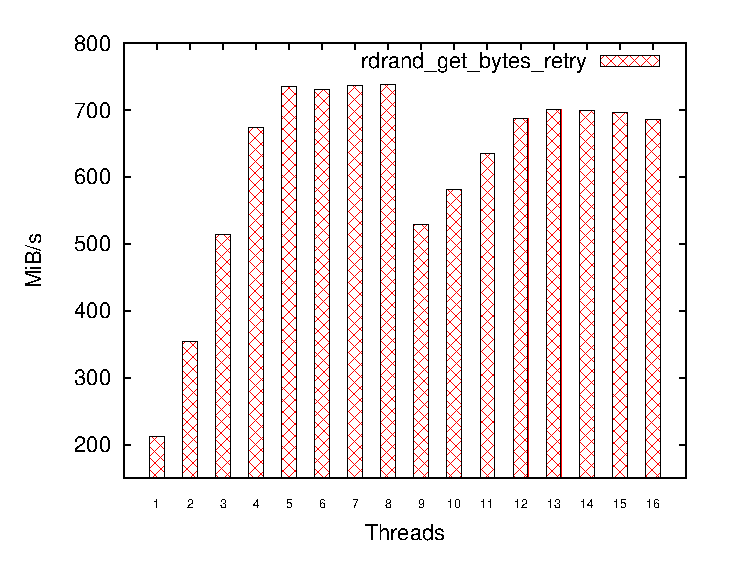
\includegraphics[width=12cm]{fig/tests/threads_scalability.eps} % Or .pdf
\caption{Amount of generated bytes in dependency of threads count.}
\label{fig:testing:threadsScalability}
\end{figure}

The speed 730 MiB/s is equal to $\frac{730 \times 2^{10} \times 2^{10}}{10^6}=765$ Hz. This is similar to the ideal 800 Hz value given in the \fullref{sec:ISK-physical}.


\subsection{Size dependency}
In this test, functions \function{rdrand_get_bytes_retry} and \function{rdrand_get_uint64_array_retry} were compared in different sizes of the memory area that was filled with random numbers. The used command is {\tt ./RdRand -m METHOD -t 1 -c SIZE} -- the test was done with a single thread and on the \machine{hp-aladdin-01.lab.bos.redhat.com} machine. For a better visibility, the figure is splitted to two parts. The figure~\ref{fig:testing:bytesArrayHi} shows the difference from 8192 down to 64 of 64-bit numbers (quadwords) and figure~\ref{fig:testing:bytesArrayLow} shows the rest, from 32 to just 1 generated number.

\begin{figure}[h!]
  \centering
 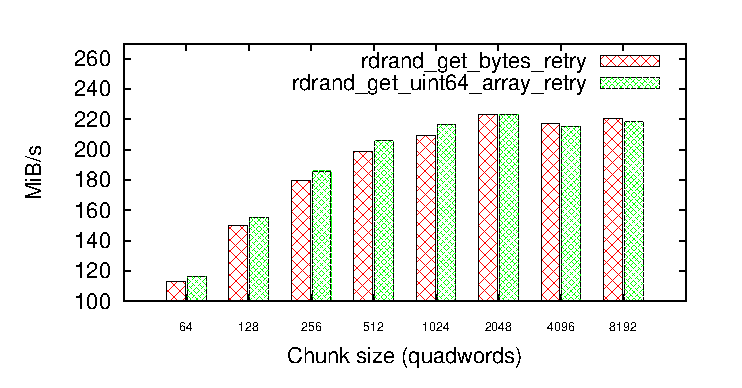
\includegraphics[width=12cm]{fig/tests/bytes_array_speed_hi.eps} % Or .pdf
%\includegraphics[width=10cm,keepaspectratio]{fig/ISK-scheme}
\caption{The difference of two functions on different sizes of filled memory area, from 8192 to 64 quadwords.}
\label{fig:testing:bytesArrayHi}
\end{figure}

\begin{figure}[h!]
  \centering
 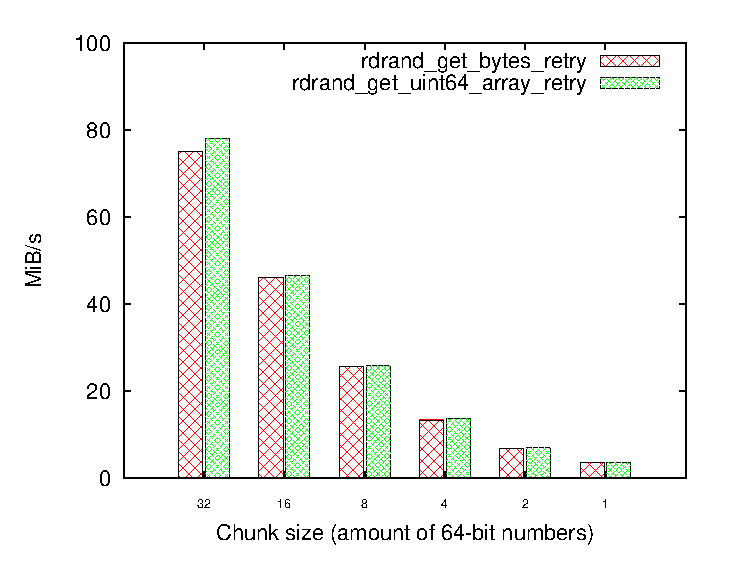
\includegraphics[width=12cm]{fig/tests/bytes_array_speed_low.eps} % Or .pdf
%\includegraphics[width=10cm,keepaspectratio]{fig/ISK-scheme}
\caption{The difference of two functions on different sizes of filled memory area, from 32 to 1 quadword.}
\label{fig:testing:bytesArrayLow}
\end{figure}

On these figures it is apparent that there is a small difference between these two values in range from very few quadwords up to about one thousand of quadwords. The difference is caused by the little higher overhead in the memory align checks in \function{rdrand_get_bytes_retry}. On very small sizes, the overhead of the test itself is too big in comparison with the difference and thus these results are not reliable. However, with regard to the implementation it is probable that the difference there still is.

On the opposite side of the figures the performance difference dismiss as with big memory areas, the overhead in the logic of the function is fractional in comparison with time spend on the RdRand instruction itself.

%\pagebreak
\subsection{Fast and secure generating}\label{subsec:testing:fastVsSecure}
Because the secure methods, described in the section \ref{subsec:api:secure}~\nameref{subsec:api:secure} (both functions \function{rdrand_get_uint64_array_reseed_delay} and its {\tt \_skip} twin), should not be used in parallel threads\footnote{See \ref{subsec:api:secure}}, only a single thread comparison between them and the \function{rdrand_get_bytes_retry} as a fast method was made. \TODO{Data from another machine that has different delay/skip.}

\begin{table}[h!]
\begin{center}
\begin{tabular}{|l|c|c|}
  \hline
 Function / Machine & \machine{hp-aladdin-01.lab.bos.redhat.com} & xx\\
  \hline
  Fast & 212.806 MB/s & xx\\ 
  \hline
  Delay & 0.116 MB/s & xx\\
  \hline
  Skip & 0.224 MB/s & xx \\
  \hline
\end{tabular}
\caption{Comparison of speed of a fast method of generating ({\tt rdrand\_get\_bytes\_retry}) and two variants of secure generating.}
\label{tab:testing:fastAndSecure}
\end{center}
\end{table}


\subsection{32 and 64-bit difference}\label{subsec:testing:32vs64}
A short comparison of performance on 32 and 64-bit system was made.
On machine \machine{hp-aladdin-01.lab.bos.redhat.com}, RHEL 5 was installed in both 32 and 64-bit version and the library was tested. As the figure~\ref{fig:testing:32vs64} shows, the performance of 32-bit version is about half of 64-bit, which is exactly in expectations based on the~\fullref{sec:ISK-physical}.

During the first stages of development we thought that the multiple variants of the RdRand instruction (16, 32 and 64-bits) were created primary because of performance, to avoid wasting of generated bits. But performance testing and finding of some more documents about Intel Secure Key showed that the these variants are there probably just for compatibility with non 64-bit operating systems and for programmer's comfort. As it is described in \fullref{subsec:DRBG}, 64 bits are always used internally.

\begin{figure}[h!]
  \centering
 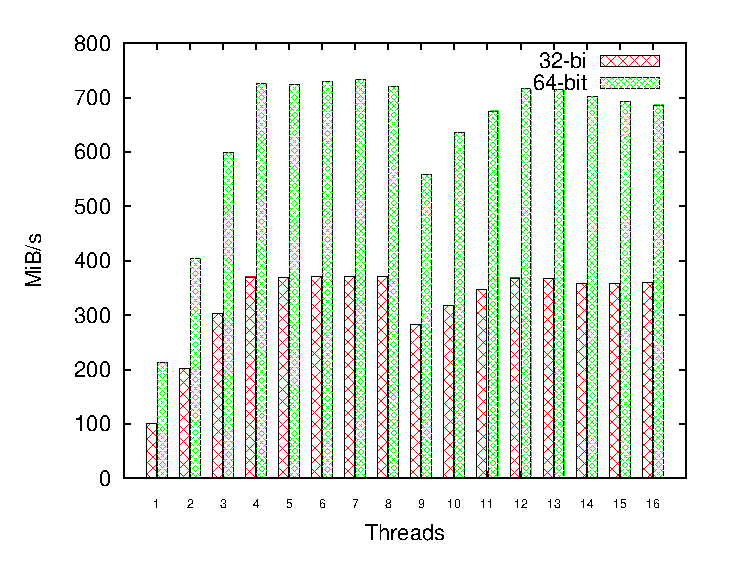
\includegraphics[width=12cm]{fig/tests/32-64bit.eps} % Or .pdf
%\includegraphics[width=10cm,keepaspectratio]{fig/ISK-scheme}
\caption{The difference between 32 and 64-bit installation}
\label{fig:testing:32vs64}
\end{figure}

\pagebreak
\subsection{Performance on an unaligned memory space}
\subsection{Half performance on some machines}

\subsection{Underflow}
The only machine on which I was able to achieve underflow of the HW RNG is \machine{dell-pr1700-02.lab.bos.redhat.com}.


\subsection{Specifications of referenced machines}
\TODO{More HW description} % TODO More HW description.

\machineDeclare{dell-pr1700-02.lab.bos.redhat.com}{Intel(R) Xeon(R) CPU E3-1285 v3 @ 3.60GHz}{Dell Precision T1700, 4 GB RAM. The internal RNG was not able to handle more than four parallel threads at November 2013.}


\machineDeclare{hp-aladdin-01.lab.bos.redhat.com}{Intel(R) Core (TM) i7-3920XM CPU @ 2.90GHz}{HP elitebook 8770w, 4 GB RAM}



%=========================================================================